Se para todo enquadramento existe um transbordamento (\cite{callon_markets_1998}), é exatamente nas bordas onde se encontra nosso interesse de estudo. Na definição não trivial, maleável e instável de fronteiras, onde cotidianamente narrativas são configuradas e reconfiguradas no ecossistema da enciclopédia. Um exemplo prático que podemos brevemente citar, para ilustrar ao leitor o local de definição de fronteiras que nos interessa, é a controvérsia em torno da política editorial de verificabilidade da Wikipédia lusófona. Ela enuncia que ``\textit{pessoas lendo e editando a enciclopédia podem checar se a informação provém de uma fonte confiável. A Wikipédia não publica pesquisa inédita; todo seu conteúdo é determinado pela informação previamente publicada ao invés de se basear apenas nas opiniões, crenças e experiências de seus editores. Mesmo se você tem certeza de que algo é verdadeiro, isto deve ser verificável através das fontes da informação antes de você adicioná-lo}'' (\citewiki{ptwiki_verificabilidade}).

Mesmo que aparentemente formulada de forma ``clara'' e ``direta'', esta regra tem suas fronteiras de aplicação constantemente movimentadas por seus/suas usuários/as, que disputam incessantemente contornos entre noções de conformidade, bom senso, respeito e qualidade.

No contexto desta disputa foi criado, em 2011, o ensaio ``\textit{Você não precisa citar que o céu é azul}''. Dissertando sobre a política de verificabilidade, afirma que ``\textit{muitos editores não entendem corretamente a política de citação, e veem nela um mecanismo para obrigar, consolidar ou deixar dúvidas sobre um ponto de vista em particular em uma disputa, ao invés de usá-la apenas para validar a informação da Wikipédia. Isto acaba gerando diversas formas de comportamentos desestabilizadores que devem ser evitados}'' (\citewiki{ptwiki_nao_precisa_citar_ceu_azul}).

Logo após criado, o ensaio viu sua página de discussão ser palco de um acalorado debate, com mais de 46 mensagens feitas por 17 diferentes usuários/as, variando de discordâncias enfáticas a apoios ao ensaio ser tornado uma política oficial. As discordâncias ganharam robustez com a publicação de outro ensaio, em 2013, intitulado ``\textit{É preciso citar que o céu é azul}''. Neste novo ensaio, defende-se que ``\textit{alguns editores podem disputar factos\footnote{Os textos da Wikipédia lusófona podem ser escritos em qualquer das diversas versões do português. Optamos por manter a grafia original das passagens transcluídas e não as adaptar para o português brasileiro.} aparentemente simples e óbvios. Até mesmo a afirmação de que ‘o céu é azul’ pode ser questionada porque o céu muito frequentemente tem cores diferentes, e todas as informações prováveis de vir a ser disputadas precisam de fontes}'' (\citewiki{ptwiki_e_preciso_citar_ceu_azul}). O ensaio ainda acrescenta que o verbete ``\textit{Céu}'', desde 2008, apresenta como legenda de sua figura principal o seguinte texto: ``\textit{quando visto de uma certa altitude, como de um avião, o céu varia de cor}'' (\citewiki{ptwiki_ceu_definicao}).

\begin{figure}[H]
    \centering
    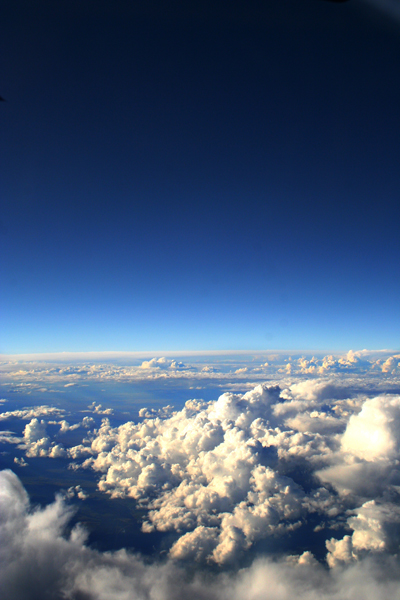
\includegraphics[width=0.4\textwidth]{Images/ceu.png}
    \caption{Imagem que ilustra o verbete “Céu” desde 2008.}
    \label{fig:ceu}
\end{figure}

Seguindo esta linha argumentativa, o ensaio conclui com as seguintes palavras: “\textit{Só porque uma coisa a si lhe parece óbvia, não significa que seja óbvia para toda a gente. Construa artigos unicamente a partir de fontes fiáveis de autoridades no assunto e cite essas fontes}” (\citewiki{ptwiki_e_preciso_citar_ceu_azul}).

Ambos os ensaios estão marcados com a predefinição ``Ensaio contestado'', que anuncia em uma caixa no topo das páginas de ambos ensaios: ``\textit{\textbf{Atenção}: Esta página contém um ensaio da Wikipédia que é seguido por parte dos seus editores, \textbf{mas é contestado por outro grupo de editores}}''\footnote{Grifos do original.} (\citewiki{ptwiki_predifinicoes_ensaios_contestado}). Ou seja, mesmo o primeiro ensaio tendo sido criado em 2011 e o segundo em 2013, até hoje, em 2020, nenhum deles foi reconhecido como uma política oficial da Wikipédia em português, e ambos contam com correligionários/as que convivem na enciclopédia com práticas antagônicas de aplicação da política de verificabilidade.

\begin{figure}[H]
    \centering
    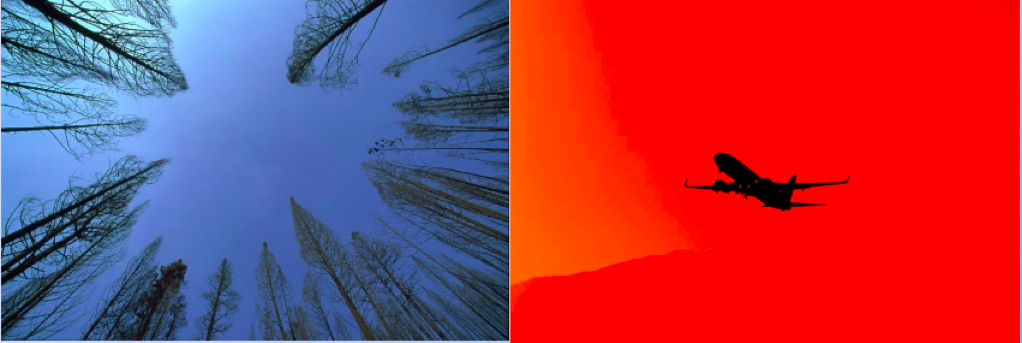
\includegraphics[width=1\textwidth]{Images/ceus-verificabilidade.png}
    \caption{Imagens que ilustram os ensaios que debatem as fronteiras de aplicação da política de verificabilidade.}
    \label{fig:ceus-verificabilidade}
\end{figure}

Situações como a relatada levaram nossa pesquisa a se interessar tanto pelos enredamentos que configuram a governança cotidiana da enciclopédia como pela forma que orientações nada triviais, como a demonstrada, podem se tornar barreiras no caminho de novos usuários que não tenha a experiência requerida para realizar devidos desvios para poderem editar.

A forma como a ambivalência de nossa pesquisa aqui citada se desenvolvera e fora implementada é então detalhada na seção a seguir.